\documentclass{scrartcl}
\usepackage[utf8]{inputenc}
\usepackage{hyperref}
\usepackage{url}
\usepackage{natbib}
\usepackage{graphicx}
\usepackage{comment}
\usepackage[textsize=tiny]{todonotes}
\newcommand{\TODO}[1]{\todo[color=orange!40, inline]{\textbf{TODO} #1}}
\newcommand{\TODOside}[1]{\todo[color=orange!40]{\textbf{TODO} #1}}
\newcommand{\NOTE}[1]{\todo[color=green!20, inline]{#1}}
\newcommand{\NOTEside}[1]{\todo[color=green!20]{#1}}
\newcommand{\REVIEWNOTE}[1]{\todo[color=violet!20, inline]{\textbf{Review note: } #1}}

\usepackage{cleveref}

\newcommand{\emailaddr}[1]{\href{mailto:#1}{\texttt{#1}}}

\title{\LARGE
    Debate2Rescue\\
}
\subtitle{Final Report for the Intelligent System Engineering Course 2025/2026}

% Consider watching:
% https://www.youtube.com/watch?v=ihxSUsJB_14
% https://www.youtube.com/watch?v=XTFWaV55uDo

\author{
    Nicolas Amadori \\ \emailaddr{nicolas.amadori@studio.unibo.it}
    \and
    Riccardo Mazzi \\ \emailaddr{riccardo.mazzi@studio.unibo.it}
    \and
    Denise Nanni \\ \emailaddr{denise.nanni@studio.unibo.it}
}

\date{\today}

\begin{document}

\maketitle

\begin{abstract}
\TODO{abstract}
\end{abstract}

\section*{AI Disclaimer}

During the preparation of this work, the authors used LLMs to help the development and to fix grammar errors in the report.

After using these tools/services, the authors reviewed and edited the content as needed and take full responsibility for the content of the final report and artifact.

\section{Introduction}

When several emergencies break out in the same area, the rescuers handling them sometimes need the same scarce resources, such as an ambulance or a helicopter, and someone has to decide who is served first and who waits.

A simple way to make this decision is to reduce every request to a number, like a fixed priority score based on the emergency data of each rescuer, and to serve the highest one.
It is fast, but the number alone does not show which aspect of the emergency produced it, and the rescuers who handle an exception cannot argue for it~\citep{rahwan2003}. %TODO: why cite here?
Consider two medical emergencies that both want the only free ambulance: the first has already been turned down more times, while the second involves a critical patient and the first does not.
A score that weighs waiting time heavily, as one would to keep requests from being starved, sends the ambulance to the first one, meanwhile the person in critical condition keeps waiting and the second team cannot argue that being critical matters more than having waited longer, so the system has no way to weigh such an argument against the others.

Debate2Rescue explores \emph{argumentation-based negotiation}~\citep{rahwan2003} as a way to make those decisions, asking agents to back their requests with reasons drawn from their emergency, such as its severity or how many times the request has already been denied.
When several agents want the same resource, they debate over multiple rounds, challenging each other on these reasons and withdrawing when nothing they can add would help.
A shared set of domain rules, evaluated after every move, decides which request currently prevails.
In the example above, the rules give the ambulance to the second emergency even though it has waited less, and the arguments that won the debate explain the choice.

The project is a multi-agent system that simulates an area where natural and human-caused emergencies arise: a rescuer agent is sent to each emergency and, once on site, requests the resource it needs, which a pilot agent then brings to the scene.
A central orchestrator dispatches the rescuers, mediates resource conflicts, and it starts a debate only when there are not enough units to satisfy every request.
All agents are BDI agents written in Jason, and the debates are evaluated with the Arg2P argumentation framework.

\Cref{sec:lit_rev} gives an overview of the literature the project builds on, while \cref{sec:analysis}, \cref{sec:design}, and \cref{sec:implementation} describe the system and how it was built.
\Cref{sec:user_guide} explains how to run the project, and \cref{sec:conclusion} explores possible future work.

\section{Literature Review}\label{sec:lit_rev}

\subsection{Abstract and Structured Argumentation}

Formal argumentation largely builds on the \emph{abstract argumentation frameworks} of \citet{dung1995}, where arguments have no internal structure and a framework is a set of arguments with a binary attack relation.
A \emph{semantics} then decides which arguments can be accepted.
The grounded one, which we use to evaluate our debates, captures a sceptical reasoner and always yields a single extension, built from the unattacked arguments by repeatedly adding the ones they defend.

Abstract frameworks do not say how arguments are built or why they attack each other.
\emph{Structured} argumentation fills this gap by building arguments from strict and defeasible rules, so that attacks follow from their structure.
An argument can contradict the conclusion of another one (rebutting), one of its premises (undermining), or deny that one of its defeasible rules applies (undercutting)~\citep{modgil2014aspic}.
Our debates rely on rebuttals and undercutters, while undermining plays no role.

Arg2P~\citep{calegari2022arg2p} is an ASPIC+-like system built on top of 2P-Kt.
Rules are written in a Prolog-like syntax and preferences between them are stated through a superiority relation.
The resulting graph is evaluated with a labelling semantics, which marks each argument as accepted (\texttt{IN}), rejected (\texttt{OUT}) or undecided (\texttt{UND}).
Its authors present it as a lightweight library, meant to be embedded in a larger system and called only where reasoning is needed.
Since it is built on logic programming, its conclusions can be traced back to readable rules, which the authors see as a way to meet explainability requirements.

\citet{pisano2021preferences} make preferences \emph{defeasible} in Arg2P, so that they are themselves conclusions of arguments and can be attacked.
In this project, preferences are fixed, and the exceptions that depend on the context are modelled as undercutters rather than as arguments about preferences.

\subsection{Argumentation in Multi-Agent Systems}

\citet{calegari2022arg2p} observe that the abstract argumentation perspective tends to see argumentation as a one-sided process in which a single party justifies a claim, while in practice it is usually an exchange between several contributors, as in multi-agent systems.
\citet{rahwan2003} survey \emph{argumentation-based negotiation}, where agents with conflicting interests, typically competing for scarce resources, exchange arguments that justify their stance or try to influence the others.
They contrast it with game-theoretic and heuristic approaches, in most of which agents can only exchange proposals and accept or reject them.
Their conceptual framework fits our design, with custom performatives as the communication language, the orchestrator's turn-taking as the protocol and the agents' beliefs as information stores.
Among the open problems, the survey asks whether a mediator should merely assist the negotiators or be able to enforce its will.
Our orchestrator operates as an in-between, as it runs the turns and hands out the resource, but the winner follows from the shared rules and the other rescuers' withdrawals.

\subsection{BDI Agents and Jason}

The belief-desire-intention (BDI) model describes an agent through what it believes about the world, the goals it wants to achieve and the plans it commits to.
\citet{bordini2007} present Jason, an interpreter for an extended version of AgentSpeak.
Jason agents react to changes in their beliefs and goals by selecting plans from a plan library, and communicate through speech-act messages whose performatives, such as \texttt{tell} or \texttt{achieve}, define the effect on the receiver.
This effect is itself defined by AgentSpeak plans, which can be overridden to handle new performatives.
The language can also be extended with internal actions, Java classes that can be called from plans and rules, where they behave like predicates.
They are our bridge to Arg2P, which the orchestrator queries to evaluate the debate and the rescuers to pick their moves.

\section{Analysis}
\label{sec:analysis}
\subsection{Problem Domain and Motivation}
\label{subsec:problem_domain}

Urban disaster response requires managing dynamic emergencies across a 2D grid containing obstacles, base stations, and mobile responders. The primary challenge is \emph{resource contention}: while field rescuers perform initial on-site triage, resolving incidents requires scarce specialized units (such as fire trucks, ambulances, or hazmat teams) that competing emergencies must share.

Standard allocation strategies like First-Come-First-Served or static scoring either ignore urgency or rely on opaque numerical formulas. Instead, \textsc{Debate2Rescue} models allocation as an argumentation process. Rescuers evaluate different conditions, including severity, victim counts, trapped individuals, and deliberate using \textsf{Arg2P}. Formal domain rules and exceptions resolve conflicts under grounded semantics, assigning the contested resource to the most justified claim.

% -----------------------------------------------------------------------------
\subsection{System Roles and Responsibilities}
\label{subsec:system_roles}
% -----------------------------------------------------------------------------

The system identifies four primary roles, each associated with specific duties:

\begin{enumerate}
    \item \textbf{Orchestrator Agent:} Coordinates the overall response. Its duties include dispatching available rescuers to newly detected incidents, collecting incoming resource requests, moderating argumentative debates when resources are contested, and granting units to the winning emergency.

    \item \textbf{Rescuer Agent:} Acts as an on-site first responder. Its duties include traveling to the incident scene, assessing local conditions (such as urgency, victims, and potential hazards), requesting the required specialized equipment, and defending the emergency's claim during resource debates.

    \item \textbf{Pilot Agent:} Operates specialized vehicles and equipment (such as fire trucks, ambulances, or hazmat units). Its duties include deploying to an incident when assigned, executing the physical rescue operation until the emergency is resolved, and returning to base.

    \item \textbf{Simulation Operator (User):} The human supervisor who oversees the simulation. The operator's duties include configuring the initial environment, adjusting simulation parameters at runtime, and monitoring agent behavior and debate outcomes.
\end{enumerate}

% -----------------------------------------------------------------------------
\subsection{Functional Requirements}
\label{subsec:functional_requirements}
% -----------------------------------------------------------------------------

The functional requirements describe the core features and operations that the system must support:

\begin{itemize}
    \item \textbf{Environment Simulation:} The system simulates a 2D grid world containing obstacles, stations, and emergencies across all the categories, each initialized with its information.
    
    \item \textbf{Emergency Dispatch:} The orchestrator automatically assigns the nearest available rescuer to new emergencies. The rescuer navigates to the incident cell, inspects local conditions to discover attributes, and requests the appropriate specialized resource.
    
    \item \textbf{Request Window:} When resource requests arrive, the orchestrator collects them within a short time window. If the number of competing requests exceeds available units, a debate is opened; if units are sufficient, they are granted directly.
    
    \item \textbf{Argumentation-Based Deliberation:} Contending rescuers participate in a turn-based dialogue using custom performatives. Moves are evaluated via \textsf{Arg2P} using grounded semantics to determine the winning emergency based on explicit domain rules and exceptions.
    
    \item \textbf{Rescue Execution and Agent Lifecycle:} The granted pilot travels to the incident and executes the rescue. Once resolved, the emergency is removed, and both responders return to base to become available again. Denied contenders retain their requests for subsequent allocation rounds.
    
    \item \textbf{GUI and Runtime Control:} The interface provides a live visual grid with tooltips and dynamic sliders allowing the operator to adjust simulation speed, spawn rate, and emergency limits during execution.
    
    \item \textbf{Audit Logging:} The system logs all simulation events in real time and automatically exports complete debate transcripts to disk, recording every move, intermediate status, and the final justification.
\end{itemize}

% -----------------------------------------------------------------------------
\subsection{Non-Functional Requirements}
\label{subsec:non_functional_requirements}
% -----------------------------------------------------------------------------

The non-functional requirements define the quality attributes and operational constraints of the application:

\begin{itemize}
    \item \textbf{Explainability:} Every allocation decision must provide an explicit, rule-based chain of arguments, clearly showing which criteria or exceptions decided the outcome.
    
    \item \textbf{Fairness:} Lower-priority emergencies must not be starved indefinitely. Each denial increases an emergency's accumulated waiting weight, allowing older requests to eventually take precedence over higher-severity but newer incidents.
    
    \item \textbf{Performance:} Deliberation through \textsf{Arg2P}, pathfinding, and visual updates must execute with minimal latency, ensuring a smooth simulation loop and a responsive user interface.
    
    \item \textbf{Concurrency and System Integrity:} State changes---such as rescuer assignments and pilot grants---must be thread-safe and atomic to prevent race conditions across parallel agent threads.
    
    \item \textbf{Observability:} The interface must make system behavior easy to understand and follow.
    
    \item \textbf{Portability:} The project must run reliably across major desktop operating systems, without requiring manual external dependencies.
\end{itemize}

\section{Design}
\label{sec:design}

\subsection{Architecture}
\label{subsec:architecture}

The system consists of a multi-agent architecture designed to separate the physical simulation environment, the BDI reasoning loop, and the argumentation engine.

Agent-environment interaction follows the standard perception-action loop: agents receive environmental percepts and perform physical actions. Agent coordination is realized through asynchronous messages using both standard and custom performatives designed for argumentation dialogues.

The architecture consists of five main layers:
\begin{enumerate}
    \item \textbf{Environment and Simulation Layer (Java):} Managed by the simulation environment (\texttt{EmergencyEnvironment}) and the domain model (\texttt{SimModel}). It manages the 2D grid, obstacles, stations, and emergencies. A dedicated thread generates emergencies according to the selected spawn rates, while the environment executes agent actions and updates agent percepts.
    
    \item \textbf{MAS Infrastructure Layer (Jason):} This layer is based on the centralized Jason infrastructure declared in \texttt{debate2rescue.mas2j} and manages the execution cycle of BDI agents, scheduling plan intentions and delivering messages through the agent communication channel.
    
    \item \textbf{Agent Layer (AgentSpeak):} Defines the autonomous entities that operate in the system: the Orchestrator, Rescuers, and Pilots. Agents maintain local beliefs, react to environment percepts, and coordinate through communication protocols.
    
    \item \textbf{Argumentation Layer (Arg2P):} Implements debates argumentations using Arg2P. It evaluates argumentation theories defined in Prolog and, through the use of custom Jason internal actions, integrates the results with the BDI agents.
    
    \item \textbf{Observability and User Interface Layer (Swing):} It provides a real-time visual representation of the grid, dynamic controls for simulation parameters, an interactive debate arena, and an audit logger that persists debate transcripts to disk.
\end{enumerate}

\TODO{Add architecture diagram illustrating the interaction between the Java environment, Jason BDI runtime, Arg2P engine, and GUI.}

\subsection{Detailed Design}
\label{subsec:detailed_design}

\subsubsection{Operational Workflows}

The overall response cycle proceeds through four sequential phases:

\begin{enumerate}
    \item \textbf{Emergency Detection and Dispatch:} When an emergency appears on the grid, the orchestrator receives the corresponding percept. It identifies all idle rescuers, calculates their grid distance to the incident, and assigns the closest one. The assigned rescuer navigates step by step toward the incident location.
    
    \item \textbf{On-Site Triage:} Upon reaching the emergency cell, the rescuer invokes \texttt{start\_rescue} to uncover the specific attributes of the incident: severity level, victim count, trapped individuals, escalating danger, physical size, and collateral risk. Using a local belief table, the rescuer identify the required resource and sends a request to the orchestrator.
    
    \item \textbf{Request Window and Contention Detection:} To avoid greedy, first-come-first-served allocations, the orchestrator groups incoming requests within a short time window. Once the window closes:
    \begin{itemize}
        \item If the number of competing requests for a given resource type is less than or equal to the number of free units, the orchestrator grants the resources directly.
        \item If requests exceed the available units, resource contention occurs and the orchestrator starts a new debate.
    \end{itemize}
    
    \item \textbf{Rescue Execution:} The pilot assigned to the winning emergency travels to the site. The time required to resolve the emergency is proportional to the emergency difficulty and, once resolved, the emergency is cleared from the environment, and both the rescuer and the pilot return to their base station, informing the orchestrator that they are free. Rescuers whose claims were denied remain on-site and increment their denial counter, gaining priority in subsequent allocation rounds.
\end{enumerate}

\subsubsection{Argumentation Model and Custom Performatives}

Resource allocation disputes are solved through structured argumentation rather than numerical scoring functions.

The argumentation theory models claims, evidence, principles, and preference rules:
\begin{itemize}
    \item \textbf{Claims and Basic Ranking:} Contenders assert a claim for the resource (\texttt{claim(E)}). Claims are ranked based on a strict priority hierarchy of emergency reasons:
    \begin{center}
    \texttt{waiting} $>$ \texttt{severity} $>$ \texttt{collateral\_risk} $>$ \texttt{trapped} $>$ \texttt{escalating} $>$ \texttt{size} $>$ \texttt{victims}
    \end{center}
    Accumulated waiting time (the number of prior denials) is prioritized by default to prevent starvation. Severity is represented numerically where smaller numbers indicate higher criticality.
    
    \item \textbf{Exceptions:} To handle critical situations where default priorities would lead to suboptimal decisions, the theory defines some exception rules that undercut standard rankings:
    \begin{itemize}
        \item \texttt{life\_first}: A critical incident ($\mathrm{severity} \le 2$) undercuts the priority of waiting time of a non-critical incident.
        \item \texttt{no\_time}: An emergency that is both spreading and trapping individuals undercuts severity differences against non-critical incidents.
        \item \texttt{prevent\_catastrophe}: An incident presenting collateral risk at large scale ($\mathrm{size} \ge 2$) undercuts severity differences.
        \item \texttt{disaster\_scale}: A major disaster with large size ($\mathrm{size} \ge 2$) and multiple victims ($\mathrm{victims} \ge 3$) undercuts waiting time.
    \end{itemize}
    
    \item \textbf{Tie-Breaking:} If two claims have identical attributes and no exception applies, the older emergency ID wins.
\end{itemize}

\paragraph{Custom Performatives.}
Standard agent communication languages provide general-purpose performatives, but lack speech acts dedicated to argumentation. We extend agent communication in Jason by introducing four custom performatives handled via the \texttt{+!kqml\_received} pattern:

\begin{itemize}
    \item \texttt{argue}: Sent by the orchestrator to all contending rescuers to formally initiate a debate and broadcast the contenders' initial claims (\texttt{move(RT, M, E, claim)}) for the contested resource type.
    \item \texttt{challenge}: Sent by a rescuer on its turn to the orchestrator (and relayed to all contenders) to attack a target competitor's claim by revealing an emergency attribute and its value (\texttt{challenge(RT, Target, Reason, Value)}) where the attacker holds an advantage.
    \item \texttt{answer}: Sent by a challenged rescuer to the orchestrator (and relayed to all contenders) to defend its claim against a specific challenge move ID, either by revealing a superior value on the disputed reason or by disclosing attributes that trigger an exception undercut.
    \item \texttt{concede}: Sent by a rescuer to the orchestrator when \textsf{Arg2P} finds no admissible move that improves its position. The orchestrator removes the rescuer from the active turn rotation, notifies remaining contenders to retract the conceded claim, and marks the request as denied for the current allocation round.
\end{itemize}

\TODO{Add sequence diagram illustrating the turn-based debate dialogue between the Orchestrator and competing Rescuers.}

\subsubsection{Internal Actions}

Two custom Jason internal actions integrate \textsf{Arg2P} into the agents' reasoning cycles:

\begin{itemize}
    \item \texttt{arg.deliberate(Moves, Labels)}: Executed by the orchestrator. It builds the argumentation theory from the move history, evaluates the graph using grounded semantics, and returns the status of each claim (\texttt{in}, \texttt{out}, \texttt{und}) along with the active winning justification (\texttt{winning\_reason}).
    
    \item \texttt{arg.choose(Moves, Me, Target, Candidates, SelectedMove)}: Executed by rescuers on their turn. It selects the first candidate that strictly improves its position against the target competitor. If no candidate improves its position, the internal action fails, prompting the rescuer to send a \texttt{concede} move.
\end{itemize}

\subsection{Agent Modeling}
\label{subsec:agent_modeling}

\subsubsection{Orchestrator Agent}
\begin{itemize}
    \item \textbf{Beliefs:} Tracks detected emergencies (\texttt{emergency}), idle rescuers (\texttt{availableRescuer}), available resource units (\texttt{availableResource}), active collection windows (\texttt{window}), and debate states (\texttt{debate}, \texttt{debate\_id}, \texttt{move}, \texttt{turn}).
    \item \textbf{Plans:}
    \begin{itemize}
        \item \texttt{!assign}: Assigns available rescuers to new incidents, prioritizing the closest rescuer.
        \item \texttt{!close\_window}: Closes the request collection window and initiates resource allocation or debate.
        \item \texttt{!deliberate}: Evaluates whether a debate is needed or if resources can be granted directly.
        \item \texttt{!next\_turn} and \texttt{!give\_turn}: Coordinates turn rotation among contenders whose claims are not accepted under grounded semantics.
        \item \texttt{!grant}: Dispatches the nearest available pilot to the winning incident.
    \end{itemize}
    \item \textbf{Concurrency:} Critical plans handling resource state and debate updates are declared as atomic to ensure thread safety when concurrent events occur simultaneously.
\end{itemize}

\subsubsection{Rescuer Agent}
\begin{itemize}
    \item \textbf{Beliefs:} Stores the assigned emergency ID and location, perceived emergency facts, the required resource type (\texttt{requesting}), the accumulated denial count (\texttt{denials}), and the debate moves history.
    \item \textbf{Plans:}
    \begin{itemize}
        \item \texttt{!handle}: Receives an incident assignment, navigates to the target cell, and performs triage.
        \item \texttt{!evaluate} and \texttt{!make\_request}: Identifies the necessary specialized resource and submits the request to the orchestrator.
        \item \texttt{!your\_turn}: Activated when the orchestrator prompts the rescuer to speak. It evaluates candidate defenses or attacks via \texttt{arg.choose} and emits an \texttt{answer}, \texttt{challenge}, or \texttt{concede} message.
        \item \texttt{!go\_home}: Returns to the base station after emergency resolution and announces availability.
    \end{itemize}
    \item \textbf{Strategy:} Rescuers disclose emergency attributes incrementally only when required to counter an opponent's argument, minimizing communication overhead.
\end{itemize}

\subsubsection{Pilot Agent}
\begin{itemize}
    \item \textbf{Beliefs:} Maintains the assigned base station coordinates, its specialized resource type, and its availability status.
    \item \textbf{Plans:}
    \begin{itemize}
        \item \texttt{!start}: Initializes the agent in the environment and informs the orchestrator of its readiness.
        \item \texttt{!move\_to\_emergency}: Dispatched by the orchestrator upon winning a debate. The pilot navigates to the incident, simulates the rescue operation duration ($2 \times \mathrm{severity} + \mathrm{victims}$), resolves the emergency, signals the waiting rescuer, and returns to base.
    \end{itemize}
\end{itemize}

\subsection{Dynamic Number of Agents}
\label{subsec:dynamic_agents}

To support arbitrary configurations without manual configuration editing, the project separates agent instantiation from the static project file: only the orchestrator agent is statically declared, while rescuer and pilot agents are spawned dynamically at runtime during environment startup based on the configuration chosen by the user.

To ensure scenario validity and operational balance, the system enforces population boundaries calculated from the average grid dimension $M$ and the station count $S$:
\begin{itemize}
    \item \textbf{Rescuers:} Bounded such that $S \le \mathrm{rescuers} \le 4 \times S$. This guarantees that every base station has at least one initial rescuer, with a maximum of four rescuers per station.
    \item \textbf{Pilots:} Bounded such that $\max(S, 9) \le \mathrm{pilots} \le 4 \times S$. The lower bound of 9 guarantees that each of the nine specialized resource types (fire truck, ambulance, police car, hazmat team, bomb squad, army, excavator, police helicopter, helicopter) has at least one pilot available in the simulation.
\end{itemize}

Because dynamic agents are created after the orchestrator has started, they register through a standardized startup handshake protocol:
\begin{enumerate}
    \item Upon instantiation, the agent executes its initial goal \texttt{!start}.
    \item The agent calls an environment action (\texttt{join\_as\_rescuer} or \texttt{join\_as\_pilot}), which places the agent entity at an available base station in the grid model.
    \item The agent sends an informative message to the orchestrator:
    \begin{center}
    \texttt{.send(orchestrator, tell, free(rescuer))}
    \end{center}
    for rescuers, or:
    \begin{center}
    \texttt{.send(orchestrator, tell, free(pilot))}
    \end{center}
    for pilots.
    \item The orchestrator handles these messages dynamically, registering available rescuers (\texttt{+availableRescuer(R)}) or pilots (\texttt{+availableResource(RT, P)}) into its belief base.
\end{enumerate}

This mechanism allows the system to scale to different population sizes without altering agent source code or restarting the multi-agent infrastructure.

\section{Implementation}\label{sec:implementation}

Debate2Rescue is a Gradle project in Java 21 built on the Jason interpreter (3.2.1) and the JVM distribution of Arg2P.

\subsection{Environment and Model}\label{subsec:impl_environment}

\texttt{EmergencyEnvironment} creates the rescuers and pilots at runtime, in the number chosen in the configuration dialog (\cref{subsec:initial_config}), and runs the simulation loop that spawns emergencies on the grid, an extension of Jason's \texttt{GridWorldModel}.
Emergency ids come from a counter, so a lower id always means an older emergency, and both the orchestrator and the theory use this to break ties.
The orchestrator perceives every responder and emergency, while a rescuer learns the attributes of its emergency only once it stands on it, such as its severity on the Emergency Severity Index (ESI, from 1 for the most severe to 5), the number of victims or its size.
Jason runs environment actions on several threads, so the model's methods on emergencies and responders are \texttt{synchronized}.

\subsection{The Debate Theory}\label{subsec:impl_theory}

The domain rules shared by all agents are in \texttt{debate.pl}.
They never change during a run, and the Java side only appends facts to them, \texttt{contender(E)} for each emergency still claiming the resource and \texttt{val(E, Reason, Value)} for each revealed value.
\Cref{fig:impl_theory} shows the core rules, without the helper predicates, the situations and the exceptions, which are summarised in \cref{tab:impl_exceptions}.

\begin{figure}[htbp]
\centering
\begin{minipage}{0.95\textwidth}
\footnotesize
\begin{verbatim}
claim(E) : prolog(contender(E)) => grant(E).
exclude(E1, E2) : grant(E1), prolog(contender(E2)), prolog(E1 < E2) -> -grant(E2).

compare(R, E1, E2) : val(E1, R, V1), val(E2, R, V2), prolog(beats(R, V1, V2))
    => ahead(R, E1, E2).
challenge(R, E1, E2) : val(E1, R, V1), prolog(worth(R, V1)), prolog(contender(E2)),
    prolog(E1 \== E2) => ahead(R, E1, E2).
answer(R, E2, E1) : val(E2, R, V2), prolog(contender(E1)), prolog(E1 \== E2)
    => undercut(challenge(R, E1, E2)).

rank(R, E1, E2) : ahead(R, E1, E2) => over(E1, E2).
asym(E1, E2) : over(E1, E2) -> -over(E2, E1).
beaten(E1, E2) : over(E1, E2) => -grant(E2).

sup(beaten(_, _), claim(_)).
sup(rank(R1, _, _), rank(R2, _, _)) :- stronger(R1, R2).
sup(claim(E1), claim(E2)) :- contender(E1), contender(E2), E1 < E2.
\end{verbatim}
\end{minipage}
\caption{Core rules of \texttt{debate.pl}. The situations, the exceptions and the helper predicates are omitted.}
\label{fig:impl_theory}
\end{figure}

Each contender has an initial claim to the resource, and a granted emergency excludes the younger ones, so with claims alone the oldest one wins.
An emergency gets ahead of another on a reason through \texttt{challenge} or \texttt{compare}.
A revealed value that counts as a reason, according to the helper \texttt{worth}, challenges every other contender at once.
The challenged one undercuts it by revealing its own value for the same reason, and from then on \texttt{compare} decides between the two values.
Being ahead turns into a ranking, and opposite rankings rebut each other, with the stronger reason prevailing.
Waiting is the strongest reason, followed by severity, collateral risk, trapped victims, escalation, size and victims, and putting it on top is how the fairness requirement (\cref{subsec:non_functional_requirements}) is satisfied by the theory.
An emergency with someone ranked over it loses its claim, and the arguments that used that claim to exclude younger contenders fall with it, which lets a younger emergency win.

The exceptions in \cref{tab:impl_exceptions} protect an emergency in a particular situation by undercutting a ranking against it.
They hold only while the penalised emergency is not critical, so they fall as soon as it reveals a severity of ESI 1 or 2.
\texttt{disaster\_scale} also falls when the penalised emergency is a major disaster itself.

\begin{table}[htbp]
\centering
\small
\begin{tabular}{|l|l|l|}
\hline
\textbf{Exception} & \textbf{Protected emergency} & \textbf{Blocked ranking} \\
\hline
\texttt{life\_first} & critical (ESI $\le 2$) & on waiting \\
\texttt{no\_time} & spreading (trapped and escalating) & on severity \\
\texttt{prevent\_catastrophe} & catastrophic (collateral risk, size $\ge 2$) & on severity \\
\texttt{disaster\_scale} & major disaster (size $\ge 2$, victims $\ge 3$) & on waiting \\
\hline
\end{tabular}
\caption{Exceptions of the theory, with the situation of the emergency they protect and the ranking that they undercut.}
\label{tab:impl_exceptions}
\end{table}

In the debate logged in \cref{fig:sample_debate_log}, emergency 10 takes the lead with a challenge on severity and loses it when 7 answers with the same ESI, since equal values leave the older claim ahead.
On size, 7 answers with a larger value, and 10, with nothing left that helps, concedes.

\subsection{Internal Actions}\label{subsec:impl_internal_actions}

The class \texttt{Debate} appends the facts to the rules and evaluates the theory with Arg2P under the grounded labelling.
The orchestrator calls \texttt{arg.deliberate(Moves, Labels)}, which turns the moves of a debate into facts and returns the labels of the rules as a Jason list.
Challenges and answers both become values, since for the theory they differ only in who reveals what.

The rescuers call \texttt{arg.choose(Moves, Me, Other, Candidates, Chosen)}.
It rebuilds the debate with only the two emergencies involved, adds each candidate as a hypothetical move and returns the first one that improves the position of \texttt{Me} against \texttt{Other}, measured on the rankings that are IN.
Some protected situations need two values, as spreading needs both trapped victims and escalation, so when no single candidate helps the action tries pairs, starting from those that can complete a situation and so trigger its exception, and returns the first value of the first pair that does.
If nothing helps, it fails.

\subsection{Agents}\label{subsec:impl_agents}

Requests for the same resource type are buffered by the orchestrator in a window of five steps, run as a separate intention with \texttt{!!} so that it keeps reacting while the window is open.
When it closes, the orchestrator grants the requests directly if enough pilots of the type are free, and opens a debate if only some are.
Before each turn it evaluates the debate with \texttt{arg.deliberate}, and the turn rotates among the contenders whose claim is not IN, each receiving the goal \texttt{your\_turn(RT, Target)} with an opponent to target.
Rescuers reply with the custom performatives \texttt{challenge}, \texttt{answer} and \texttt{concede}, handled through plans for Jason's \texttt{kqml\_received} goal that accept a move only from the rescuer holding the turn.
Every move is relayed to all contenders, so each rescuer keeps the same copy of the debate as the orchestrator.
When nobody is left to give the turn to, the winner gets the closest free pilot, which travels to the emergency and resolves it, while the losers are told \texttt{denied} and keep their requests pending, to be deliberated again as soon as a pilot of that type is free.

A rescuer maps its emergency onto the seven reasons of the theory, using the number of debates it has lost as its value for waiting.
On its turn it runs the plan in \Cref{fig:impl_rescuer_turn}, where \texttt{requesting} holds its request and \texttt{moves} its copy of the debate.

\begin{figure}[htbp]
\centering
\begin{minipage}{0.95\textwidth}
\footnotesize
\begin{verbatim}
+!your_turn(RT, T)[source(orchestrator)]
    : requesting(Id, RT, _) & moves(RT, Moves) <-
    if (unanswered(RT, Id, M, A, R) & answers(RT, Id, M, R, Answers) &
        arg.choose(Moves, Id, A, Answers, answer(M, R2, V))) {
        .send(orchestrator, answer, answer(RT, M, R2, V));
    } elif (challenges(RT, Id, T, Challenges) &
            arg.choose(Moves, Id, T, Challenges, challenge(T, AR, AV))) {
        .send(orchestrator, challenge, challenge(RT, T, AR, AV));
    } else {
        .send(orchestrator, concede, concede(RT));
    }.
\end{verbatim}
\end{minipage}
\caption{The plan of \texttt{rescuer.asl} that picks the rescuer's move on its turn.}
\label{fig:impl_rescuer_turn}
\end{figure}

The rescuer first tries to answer a challenge it has not answered yet, offering its value for that reason and then its other unrevealed values, since a different value can trigger an exception.
Otherwise it challenges its target with its unrevealed values from the strongest reason down, and if nothing helps it concedes.

\subsection{Logging and Testing}\label{subsec:impl_view}

The orchestrator logs every debate through environment actions that forward the events to \texttt{DebateLogger}, which writes one file per debate (\cref{subsec:persistent_logs}) and updates the side panel.
With each status update the orchestrator logs the rank and exception rules that are IN, and the logger uses the final list as the justification of the debate or, if it is empty because the others conceded, the last reason seen during the debate.

JUnit tests cover the theory rule by rule, the move choice of \texttt{arg.choose}, the environment and the model, and a GitHub Actions workflow runs them, together with a Spotless formatting check, on every pull request towards \texttt{main} and \texttt{develop}.

\section{User Guide}
\label{sec:user_guide}

This section describes how to configure, run, and monitor the \textsc{Debate2Rescue} simulation. It details system requirements, startup configuration, the graphical user interface (GUI), runtime controls, and debate log files.

% -----------------------------------------------------------------------------
\subsection{Getting Started}
\label{subsec:getting_started}
% -----------------------------------------------------------------------------

\subsubsection{Prerequisites}
The simulation requires:
\begin{itemize}
    \item \textbf{Java Development Kit (JDK):} Version 21 or higher.
    \item \textbf{Gradle:} The repository bundles the Gradle wrapper (\texttt{gradlew}), so a separate local Gradle installation is not required.
    \item \textbf{Operating System:} Linux, macOS, or Windows with graphical desktop support.
\end{itemize}

\subsubsection{Running the Simulation}
To launch the simulation with default settings, run from the project root:
\begin{verbatim}
./gradlew run
\end{verbatim}
or on Windows:
\begin{verbatim}
gradlew.bat run
\end{verbatim}

On startup, a configuration dialog opens before initializing the agents and grid environment.

% -----------------------------------------------------------------------------
\subsection{Initial Configuration}
\label{subsec:initial_config}
% -----------------------------------------------------------------------------

The startup dialog (\texttt{SimConfigDialog}, \Cref{fig:config_dialog}) allows configuring the grid dimensions and agent population.

\begin{figure}[htbp]
    \centering
    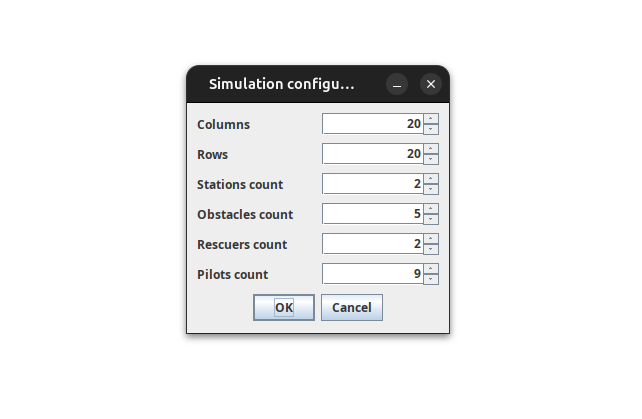
\includegraphics[width=0.45\textwidth]{figures/sim_config_dialog.png}
    \caption{Simulation configuration dialog.}
    \label{fig:config_dialog}
\end{figure}

The configurable parameters and ranges are summarized in \Cref{tab:initial_config_params}.

\begin{table}[htbp]
\centering
\small
\begin{tabular}{|l|c|c|p{5.5cm}|}
\hline  
\textbf{Parameter} & \textbf{Default} & \textbf{Range} & \textbf{Description} \\
\hline
\textbf{Columns} & 20 & 10 -- 50 & Grid width. \\
\textbf{Rows} & 20 & 10 -- 50 & Grid height. \\
\textbf{Stations} & 2 & 1 -- MaxStations & Number of base stations. \\
\textbf{Obstacles} & 5 & 0 -- MaxObstacles & Number of obstacle cells. \\
\textbf{Rescuers} & 2 & 1 -- MaxRescuers & Number of rescuer agents. \\
\textbf{Pilots} & 9 & MinPilots -- MaxPilots & Number of resource pilots. \\
\hline
\end{tabular}
\caption{Initial configuration parameters.}
\label{tab:initial_config_params}
\end{table}

\subsubsection{Validation Rules and Default Values}
The dialog enforces several constraints based on the average grid dimension $M$ based on the grid width and height:
\begin{itemize}
    \item \textbf{Base stations:} Defaults to $\mathrm{round}(0.10 \times M)$ with an upper limit of $\mathrm{round}(0.50 \times M)$.
    \item \textbf{Obstacles:} Defaults to $\mathrm{round}(0.25 \times M)$ with an upper limit of $\mathrm{round}(1.00 \times M)$.
    \item \textbf{Rescuers:} At least one rescuer per station, up to a maximum of four per station ($\mathrm{stations} \le \mathrm{rescuers} \le 4 \times \mathrm{stations}$). The default assigns one rescuer per station.
    \item \textbf{Pilots:} Bounded between $\max(\mathrm{stations}, 9)$ and $4 \times \mathrm{stations}$, ensuring that every station has at least one pilot and that each of the nine resource types (helicopter, fire truck, ambulance, police car, excavator, police helicopter, army, bomb squad, hazmat team) has an assigned pilot.
\end{itemize}

% -----------------------------------------------------------------------------
\subsection{Graphical User Interface}
\label{subsec:gui_overview}
% -----------------------------------------------------------------------------

After configuration, the main application window is displayed (\Cref{fig:main_gui}). It is divided into two sections:
\begin{enumerate}
    \item \textbf{Grid Canvas (Left):} A 2D grid rendering the environment, stationary structures, and mobile agents.
    \item \textbf{Side Panel (Right):} Hosts runtime controls, the visual legend, and two real-time logging panes.
\end{enumerate}

\begin{figure}[htbp]
    \centering
    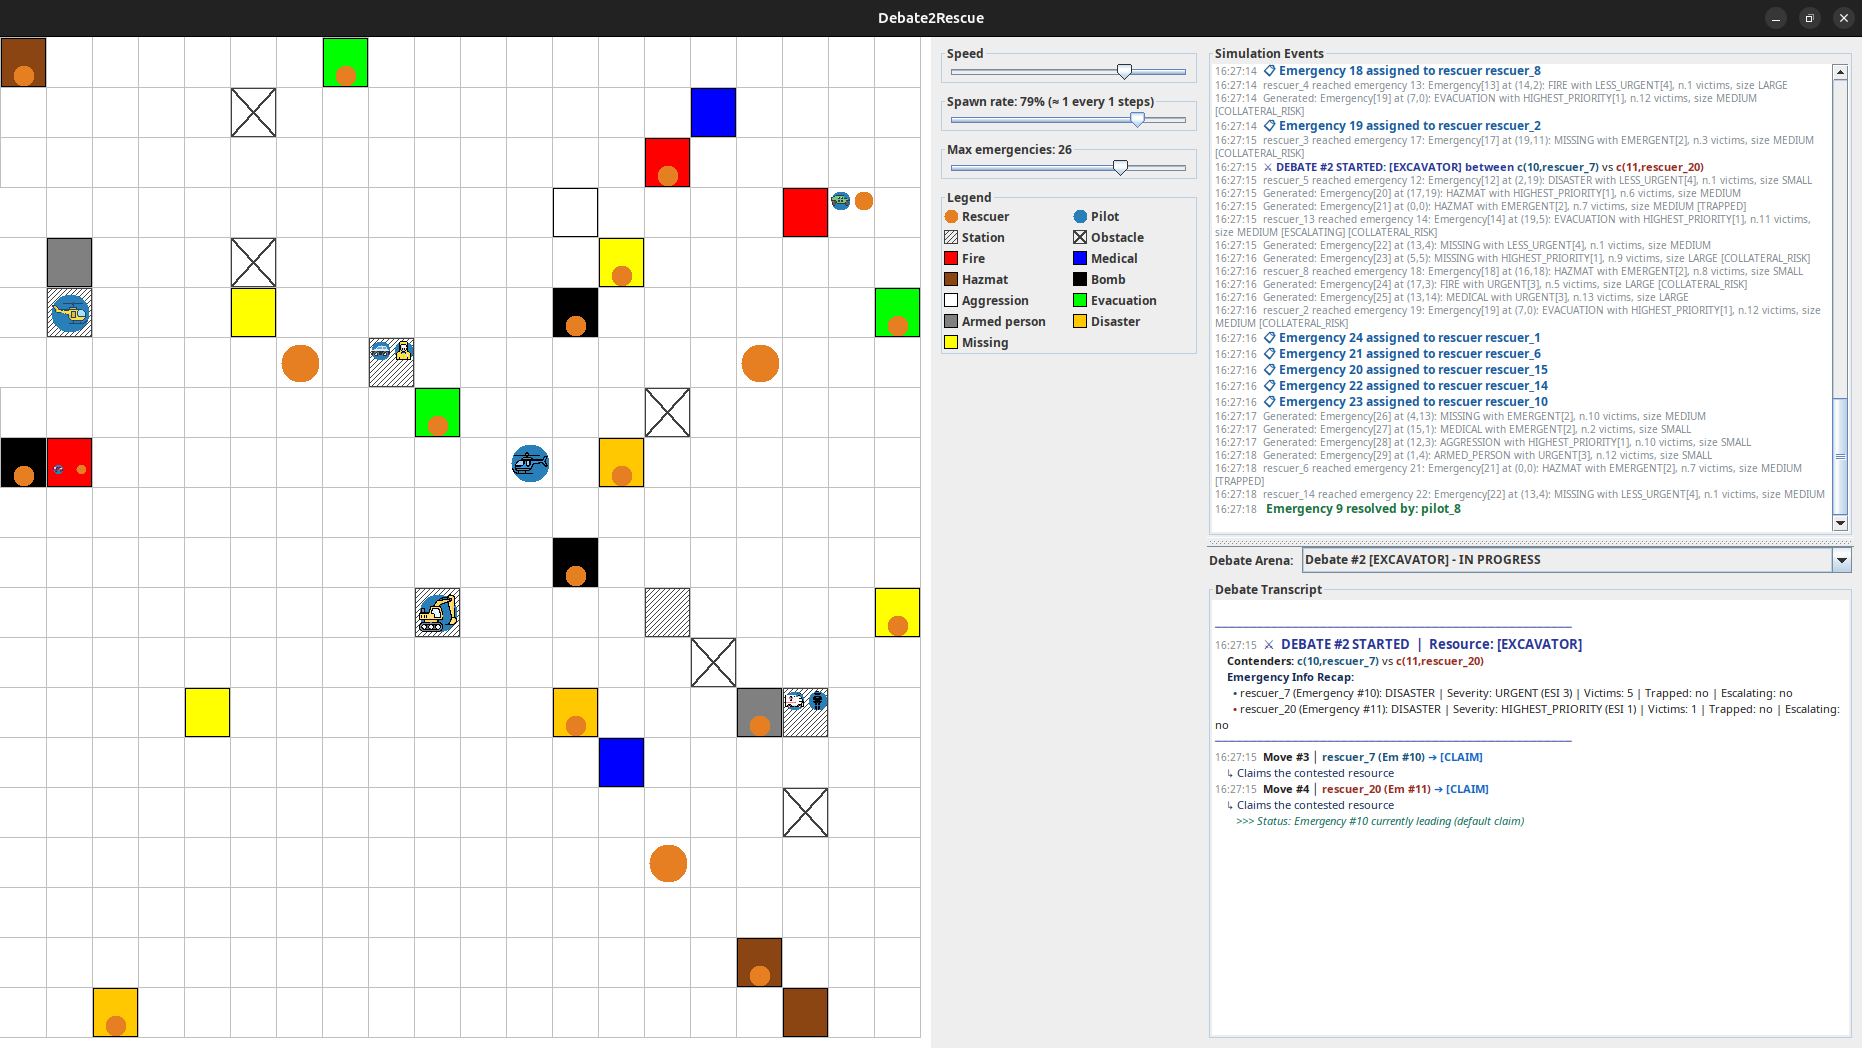
\includegraphics[width=0.95\textwidth]{figures/main_gui.png}
    \caption{The main graphical user interface of \textsc{Debate2Rescue}.}
    \label{fig:main_gui}
\end{figure}

\subsubsection{Grid Elements}
The canvas displays entities using distinct shapes and colors:
\begin{itemize}
    \item \textbf{Base Stations:} Gray cells with diagonal stripes, representing bases where responders wait between assignments.
    \item \textbf{Obstacles:} White cells with a dark cross, representing impassable cells.
    \item \textbf{Emergencies:} Colored squares, color-coded by emergency category.
    \item \textbf{Responders:} Circles representing rescuer and pilot agents, color-coded by role.
\end{itemize}
A visual legend at the bottom-left of the side panel maps each icon and color to its corresponding entity or emergency type.

\subsubsection{Cell Tooltips}
Hovering the cursor over any station or emergency cell displays a tooltip with details such as emergency status, severity level (and ESI score), victim count, station presence, and any responders currently on the cell.

% -----------------------------------------------------------------------------
\subsection{Runtime Simulation Controls}
\label{subsec:runtime_config}
% -----------------------------------------------------------------------------

Three sliders at the top of the side panel allow adjusting simulation parameters dynamically during execution (\Cref{fig:sliders}):
\begin{itemize}
    \item \textbf{Speed:} Controls step execution delay; moving the slider to the right increases simulation speed.
    \item \textbf{Spawn rate:} Controls the per-step probability of spawning a new emergency ($0\%$ to $100\%$). Setting it to $0\%$ disables new emergency generation.
    \item \textbf{Max emergencies:} Sets the upper limit on concurrent active emergencies in the grid.
\end{itemize}

\begin{figure}[htbp]
    \centering
    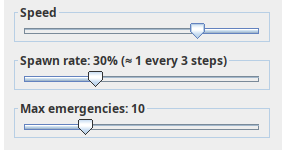
\includegraphics[width=0.4\textwidth]{figures/sliders.png}
    \caption{Runtime adjustment sliders in the side panel.}
    \label{fig:sliders}
\end{figure}

% -----------------------------------------------------------------------------
\subsection{Real-Time Logging}
\label{subsec:gui_logging}
% -----------------------------------------------------------------------------

The side panel features two vertically split logging panes: the upper pane logs general simulation events, while the lower pane streams debate transcripts.

\begin{figure}[htbp]
    \centering
    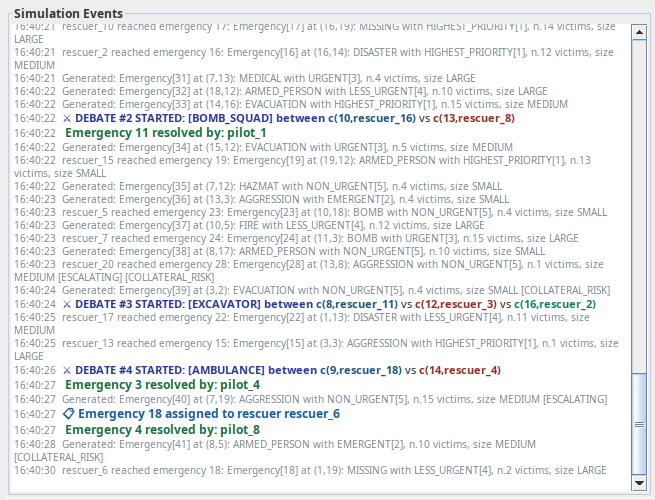
\includegraphics[width=0.55\textwidth]{figures/simulation_events.png}
    \caption{Simulation events log (top pane).}
    \label{fig:simulation_events}
\end{figure}

\subsubsection{Simulation Events Pane}
The upper pane logs environment and multi-agent lifecycle events in real time (\Cref{fig:simulation_events}):
\begin{itemize}
    \item \textbf{Routine grid events:} Actions already visible on the canvas (agent movement, emergency spawn, agent registration) are shown in muted gray to reduce clutter.
    \item \textbf{Task coordination events:} Highlighted with icons and colors:
    \begin{itemize}
        \item \texttt{[Assign]} (blue): Emergency assignment sent to a rescuer.
        \item \texttt{[Resolve]} (green): Emergency successfully resolved.
        \item \texttt{[Message]} (dark text): Direct inter-agent communication.
    \end{itemize}
    \item \textbf{Debate summaries:} One-line notices marking the start and conclusion of each resource debate, indicating the debate ID, contested resource, and winner.
\end{itemize}

\subsubsection{Debate Arena Pane}
The lower pane records the argumentation dialogue whenever two or more rescuers compete for the same specialized resource via Arg2P (\Cref{fig:debate_arena}).

\begin{figure}[htbp]
    \centering
    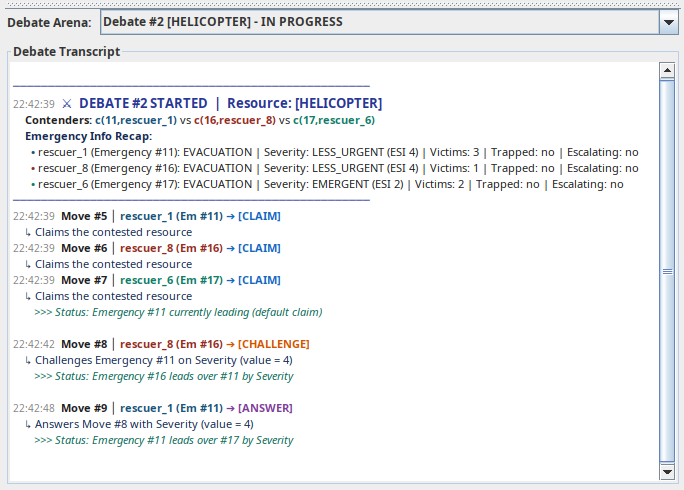
\includegraphics[width=0.55\textwidth]{figures/debate_arena.png}
    \caption{Debate arena transcript (bottom pane).}
    \label{fig:debate_arena}
\end{figure}

The Debate Arena contains:
\begin{itemize}
    \item \textbf{Session selector:} A dropdown menu to switch between active and concluded debates (most recent first).
    \item \textbf{Header:} Summarizes the contested resource and contender emergency profiles (severity, victim count, trapped victims, escalation status).
    \item \textbf{Dialogue turns:} Color-coded by performative:
    \begin{itemize}
        \item \textbf{\textcolor{blue}{CLAIM:}} Resource request by an agent.
        \item \textbf{\textcolor{orange}{CHALLENGE:}} Attack on an opponent's priority based on criteria such as severity or victim count.
        \item \textbf{\textcolor{violet}{ANSWER:}} Response or counter-argument defending an emergency.
        \item \textbf{\textcolor{red}{CONCEDE:}} Concession withdrawing a claim when an opponent's argument dominates.
    \end{itemize}
    \item \textbf{Turn status:} Updates after each move to display the current leader and the applied ranking rule.
    \item \textbf{Debate summary:} Concluding banner showing the winning emergency, the assigned rescuer, the final justification, and any conceded contenders.
\end{itemize}

% -----------------------------------------------------------------------------
\subsection{Persistent File Logs}
\label{subsec:persistent_logs}
% -----------------------------------------------------------------------------

Each debate session is saved to disk for inspection and offline analysis.

\subsubsection{Directory Structure and File Naming}
On each run, a timestamped directory is created under \texttt{logs/}:
\[
\texttt{logs/yyyy-MM-dd\_HH-mm-ss/}
\]
Each debate produces an individual log file named:
\[
\texttt{debate<ID>\_<resource\_type>.log}
\]
For example, \texttt{debate1\_fire\_truck.log}.

\subsubsection{Log File Structure}
Each log file contains three parts:
\begin{enumerate}
    \item \textbf{Header:} Start timestamp, contested resource, and contender profiles (emergency ID, severity, victim count, trapped victims, and escalation status).
    \item \textbf{Moves log:} Timestamped record of each argumentative move and the intermediate leading state with its ranking rule.
    \item \textbf{Footer:} Final decision, winner, conceded contenders, deciding justification, and total move count.
\end{enumerate}

A sample debate log is shown in \Cref{fig:sample_debate_log}.

\begin{figure}[htbp]
\centering
\begin{minipage}{0.95\textwidth}
\footnotesize
\begin{verbatim}
=================================================================
DEBATE #1 STARTED: Resource Type [fire_truck]
Timestamp: 2026-10-28 14:35:45
Contenders: c(7,rescuer_15), c(10,rescuer_13)

Contender Emergency Infos:
  * rescuer_15 (Emergency #7): FIRE | Severity: LESS_URGENT (ESI 4)
    | Victims: 12 | Trapped: no | Escalating: no
  * rescuer_13 (Emergency #10): FIRE | Severity: LESS_URGENT (ESI 4)
    | Victims: 2  | Trapped: no | Escalating: no
=================================================================

--- DEBATE MOVES & TURNS ---
[2026-10-28 14:35:45] Move #1: rescuer_15 (Emergency 7)  -> CLAIM: claim
[2026-10-28 14:35:45] Move #2: rescuer_13 (Emergency 10) -> CLAIM: claim
       >>> Status: Leading Emergency = 7 | Reason: []

[2026-10-28 14:35:54] Move #5: rescuer_13 (Emergency 10) -> CHALLENGE:
       challenge(7,severity,4)
       >>> Status: Leading Emergency = 10 | Reason: [rank(severity,10,7)]

[2026-10-28 14:36:07] Move #12: rescuer_15 (Emergency 7) -> ANSWER:
       answer(5,severity,4)
       >>> Status: Leading Emergency = 7 | Reason: []

[2026-10-28 14:36:33] Move #15: rescuer_13 (Emergency 10) -> CHALLENGE:
       challenge(7,size,2)
       >>> Status: Leading Emergency = 10 | Reason: [rank(size,10,7)]

[2026-10-28 14:37:30] Move #22: rescuer_15 (Emergency 7) -> ANSWER:
       answer(15,size,3)
       >>> Status: Leading Emergency = 7 | Reason: [rank(size,7,10)]

[2026-10-28 14:38:33] Move #30: rescuer_13 (Emergency 10) -> CONCEDE:
       "withdrew claim"
       >>> Status: Leading Emergency = 7 | Reason: []

=================================================================
DEBATE #1 CONCLUDED: Resource Type [fire_truck]
Timestamp: 2026-10-28 14:38:33
FINAL DECISION: Winner is Emergency 7
DENIED CONTENDERS: c(10,rescuer_13) [conceded]
JUSTIFICATION: All opponent(s) conceded (deciding argument: size)
TOTAL MOVES: 30
=================================================================
\end{verbatim}
\end{minipage}
\caption{Excerpt of a persistent debate log file (\texttt{debate1\_fire\_truck.log}).}
\label{fig:sample_debate_log}
\end{figure}

\section{Comments}

\bibliographystyle{plainnat}
\bibliography{biblio}

\end{document}